\section{Point Mass}
The first system model to test was the simple point mass as stated in chapter \ref{ch:Approach}.
While this implementation is a simple version it does already work surprisingly good.
The mean error over the whole flight is normally around 4-5 meter.
It has to be said that this only works while no sensor has a greater offset.
Therefore these values come at the cost that they are not that trustworthy, 
because the system noise on the acceleration has to be set to a greater value to get those good estimation.
An additional factor is also the pitch angle which does hinder this estimation if it changes in a great manner.
This can be seen in figure \ref{fig:PointMassErrorWithOffset} which shows the state estimation error with different offsets.

\begin{figure}[h!]
 \centering
 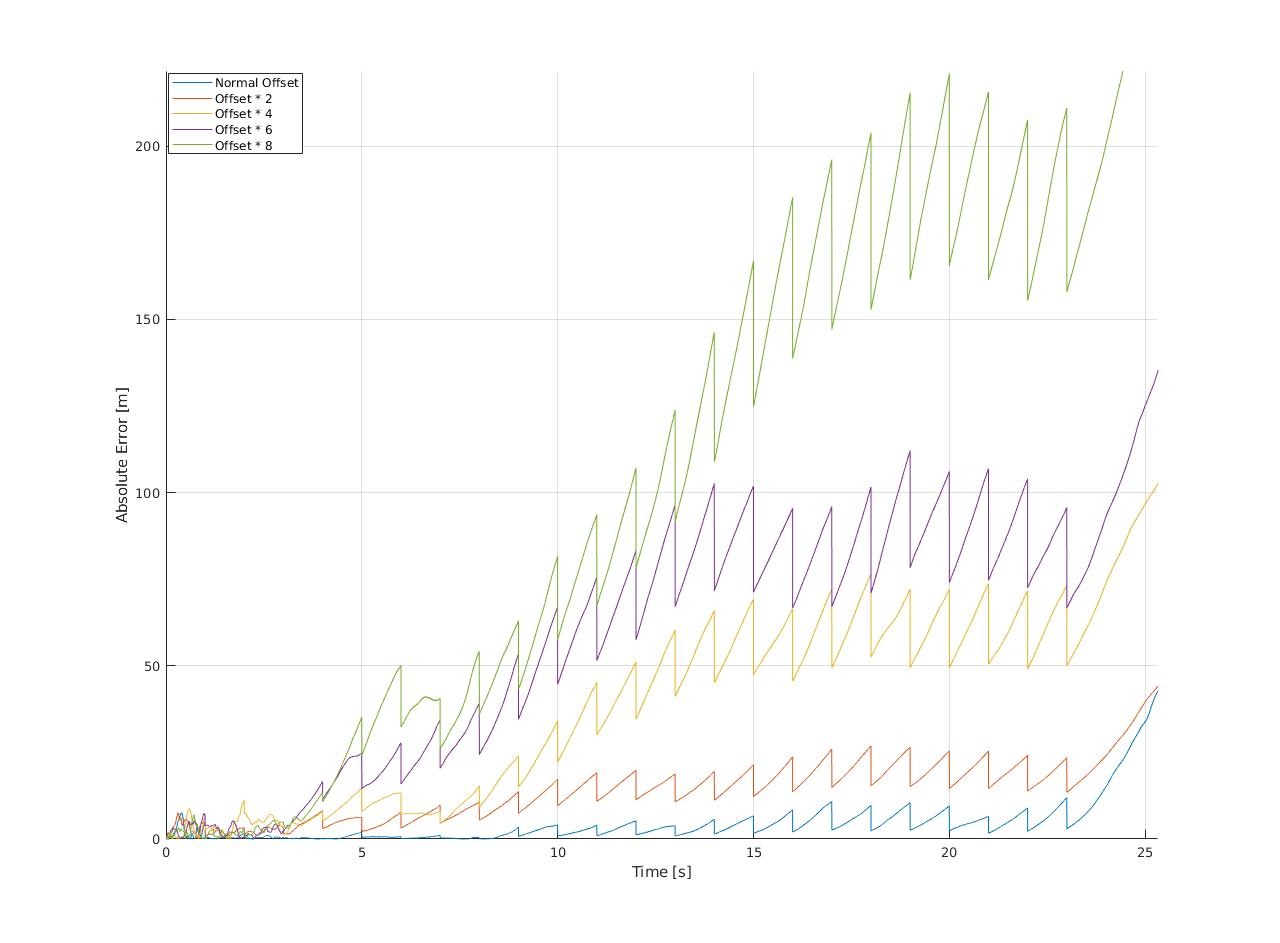
\includegraphics[width=.8\textwidth]{./Pictures/PointMassErrorWithOffset.jpg}
 % PointMassErrorWithOffset.jpg: 0x0 pixel, 300dpi, 0.00x0.00 cm, bb=
 \caption{Error during flight time with different offsets}
 \label{fig:PointMassErrorWithOffset}
\end{figure}


The table \ref{tab:PointMassPerformanceWithOffset} shows the mean and median of the error in the height depending on the offset on the accelerometer.

\begin{table}
\begin{center}
\begin{tabular}{ccc}
& Mean & Median\\
Normal & 4.57 & 2.80\\
2Times & 13.97 & 14.66\\
4Times & 39.31 & 46.99\\
6Times & 59.35 & 71.90\\
8Times & 107.21 & 102.15
\end{tabular}
\end{center}
\label{tab:PointMassPerformanceWithOffset}
\end{table}

This shows that the error which the estimator makes does rise exponentially.
So this is an issue which should be assessed by including an acceleration offset in the state vector.

\subsection{Performance}
%% Add a performance table like max min mean median error under different circumstances. With offsets 
% Discuss pros and cons like not that good estimation but small system load 


\section{Point Mass with Acceleration Offset}
While this system works also sometimes no so good as the first most times it works much better and therefore this should be implemented in the final system.
Like above the figure \ref{fig:PointMassOffsetErrorWithOffset} shows the error during a flight with different sensor offsets.
It can clearly be seen that while the mean error does rise about some value, it always get back to zero and therefore overall this system preforms better as the simple point mass.

\begin{figure}[h!]
 \centering
 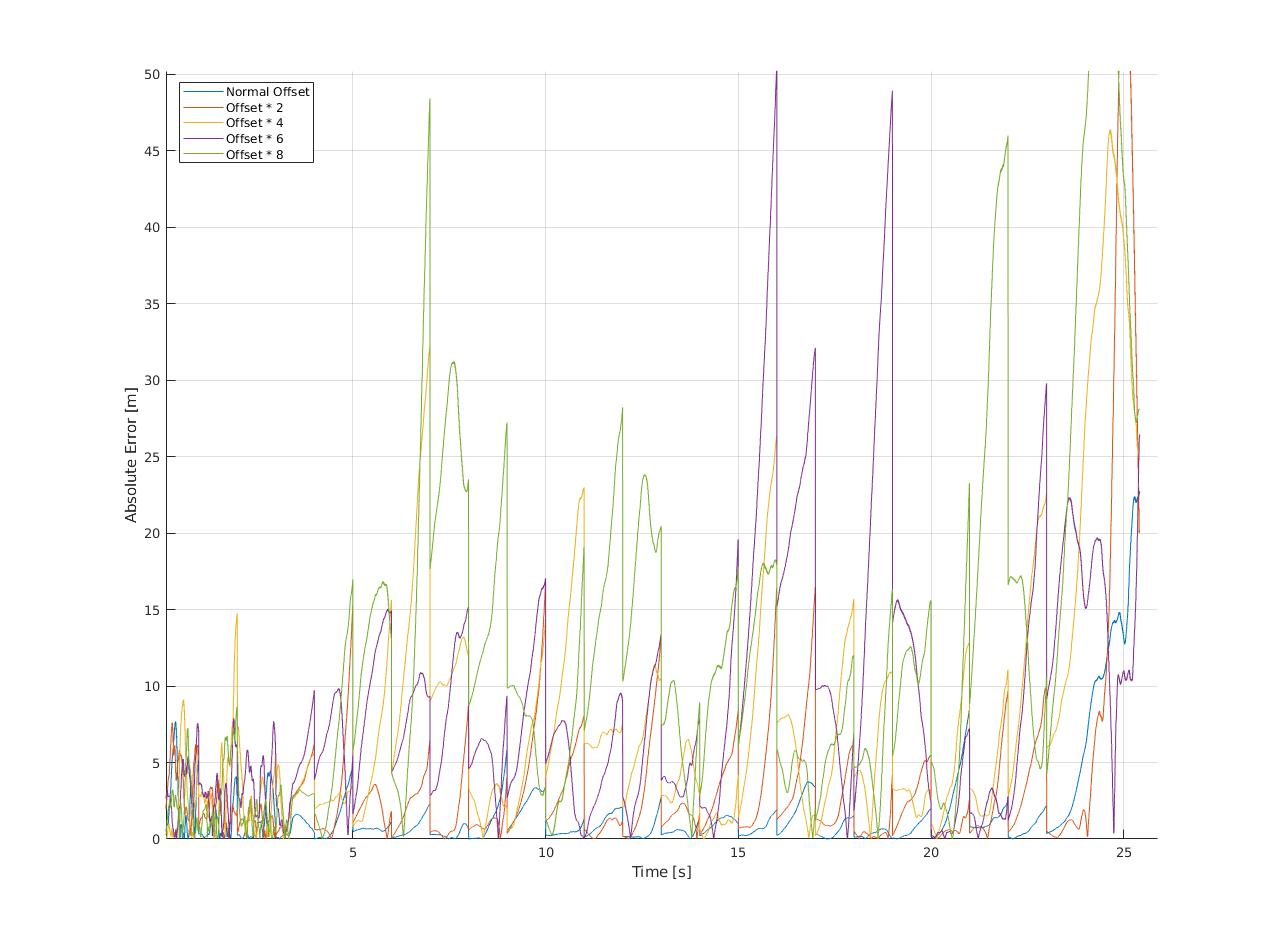
\includegraphics[width=0.8\textwidth]{./Pictures/PointMassOffsetErrorWithOffset.jpg}
 % PointMassOffsetErrorWithOffset.jpg: 0x0 pixel, 300dpi, 0.00x0.00 cm, bb=
  \caption{Error during flight time with different offsets}
 \label{fig:PointMassOffsetErrorWithOffset}
\end{figure}
 
\subsection{Performance}
%While it performes much better than the only point mass system it should be much room for above.


\section{Point Mass with Pressure}
The pressure used as state vector has to be shown that it is not that good as firstly tough.
While it does increase the accuracy it does also increase the needed computational effort due to the fact that to get a real added value from this,
the height out of the pressure has to be calculated at each time step with the help of the estimated pressure.
In addition when the temperature gradient is chosen wrong it deeply effects the estimation like seen in figure \ref{fig:PointMassVSPressure}.
The errors there were low pass filtered with an moving average filter for better visualisation.

\begin{figure}[h!]
 \centering
 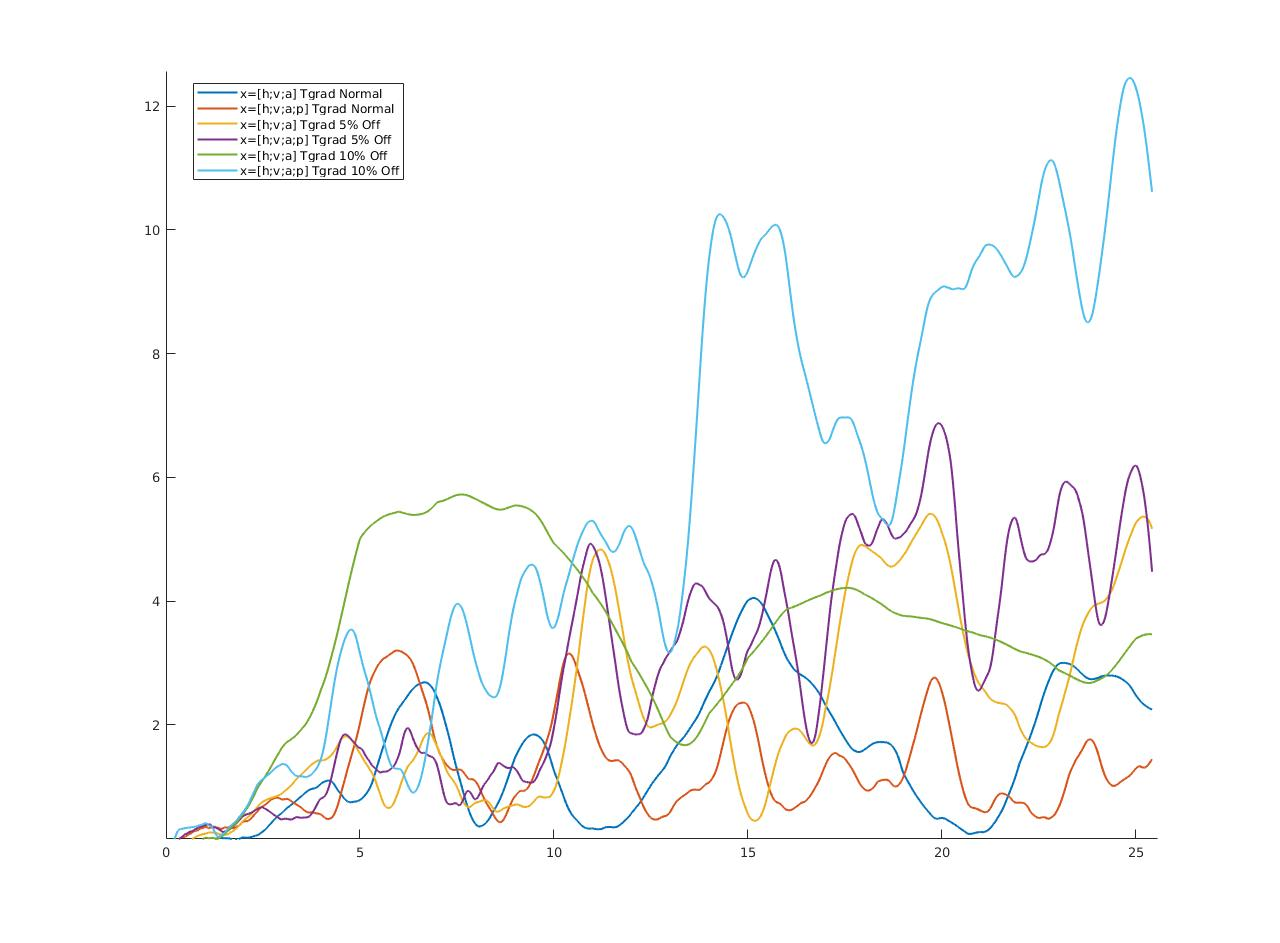
\includegraphics[width=.8 \textwidth]{./Pictures/PointMassVSPressure.jpg}
 % PointMassVSPressure.jpg: 0x0 pixel, 300dpi, 0.00x0.00 cm, bb=
 \caption{Plot of point mass vs the pressure low pass filtered}
 \label{fig:PointMassVSPressure}
\end{figure}

In this figure the error for both a system with acceleration offset (which therefore can depend more on the accelerometer measurements) is compared against the system model with the pressure in the state vector.
While they preform equal as good while the temperature gradient is determined correct.
If the gradient is determined wrong by just 5 percent it already performance less accurate than all other tested system models.
This is a problem due to the fact that the temperature gradient will most certanly not be correct during the whole flight.
With this can be seen that the system performance is more ore less the same as the normal point mass system.
Therefore the cost and problems that can occur outweight the gain here so it will not be implemented in the best system here..



\section{Point Mass with Pitch angle}
The pitch angle is difficult to estimate because it has no measured dependencies on its own.
Therefore the kalman filter does just something like a real time low pass filtering on those measurements.
So the system noise on the pitch angle has to be as good calculated as possible to optimise its estimation.
In addition the impact of the pitch angle is smaller than firstly tought.
This mainly because the pitch angle does only start to get to a greater value after the burnout.
After this the vertical acceleration is much smaller and therefore a error of the angle by a few degrees does not make such a great impact.
This can be seen in the plot of figure \ref{fig:PointMassVSPitch} where the estimation which uses the pitch angle as a state variable does only performance slightly better.
\begin{figure}[h!]
 \centering
 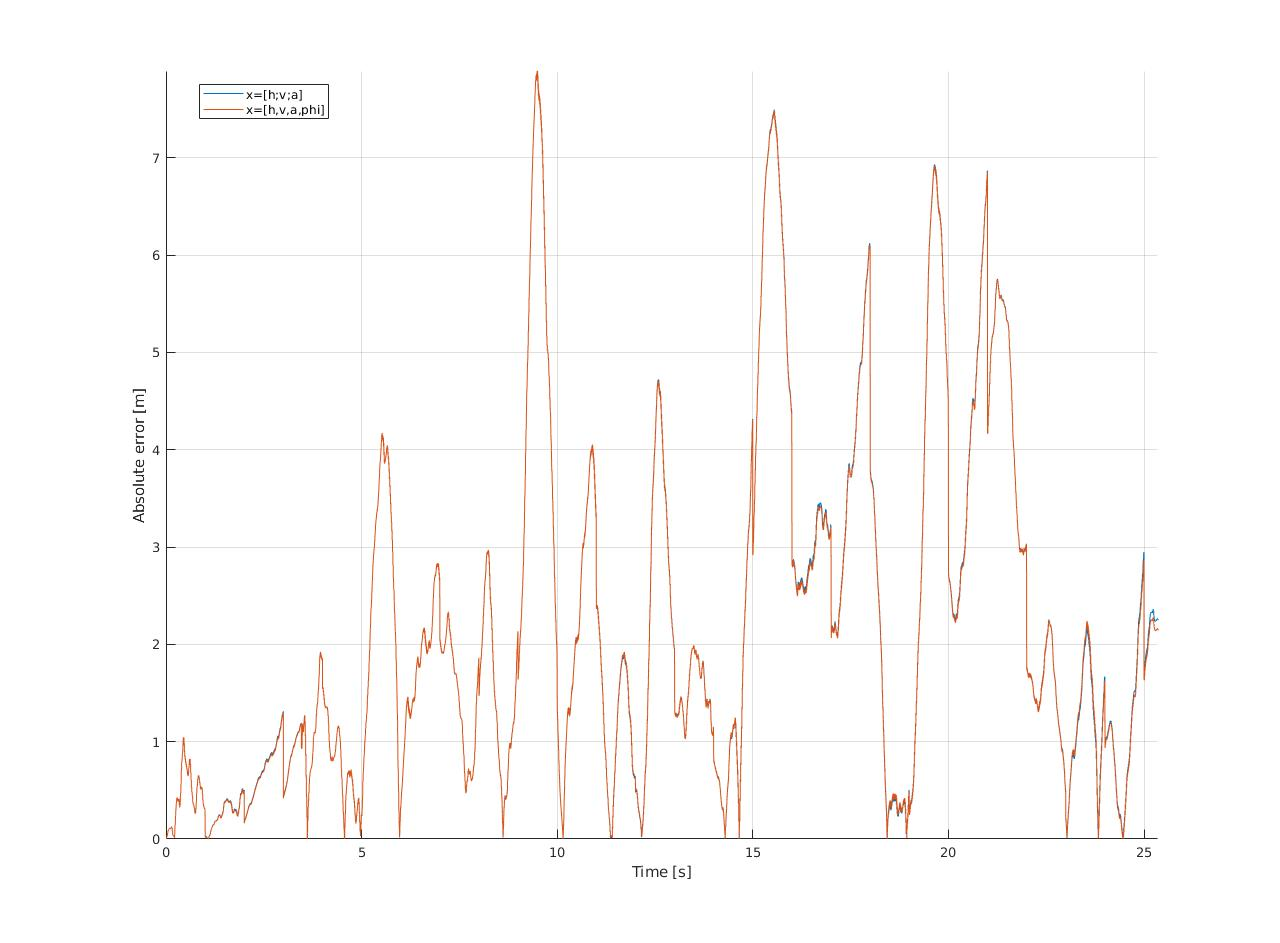
\includegraphics[width=.8 \textwidth]{./Pictures/PointMassVSPitch.jpg}
 % PointMassVSPitch.jpg: 0x0 pixel, 300dpi, 0.00x0.00 cm, bb=
 \caption{Estimation error over time from point mass system with and without pitch angle inclusion}
 \label{fig:PointMassVSPitch}
\end{figure}

On the other hand in this implementation the pitch angle does more of less the same thing as the acceleration offset because of it properties.


\section{Point Mass with Acceleration as input}
It can be seen in the plot in figure \ref{fig:PointMassVSAccelerationInput}, that the estimated height estimated when the acceleration measurements are taken as a input that they reseamble more or less the exact values as from the normal system.
\begin{figure}[h!]
 \centering
 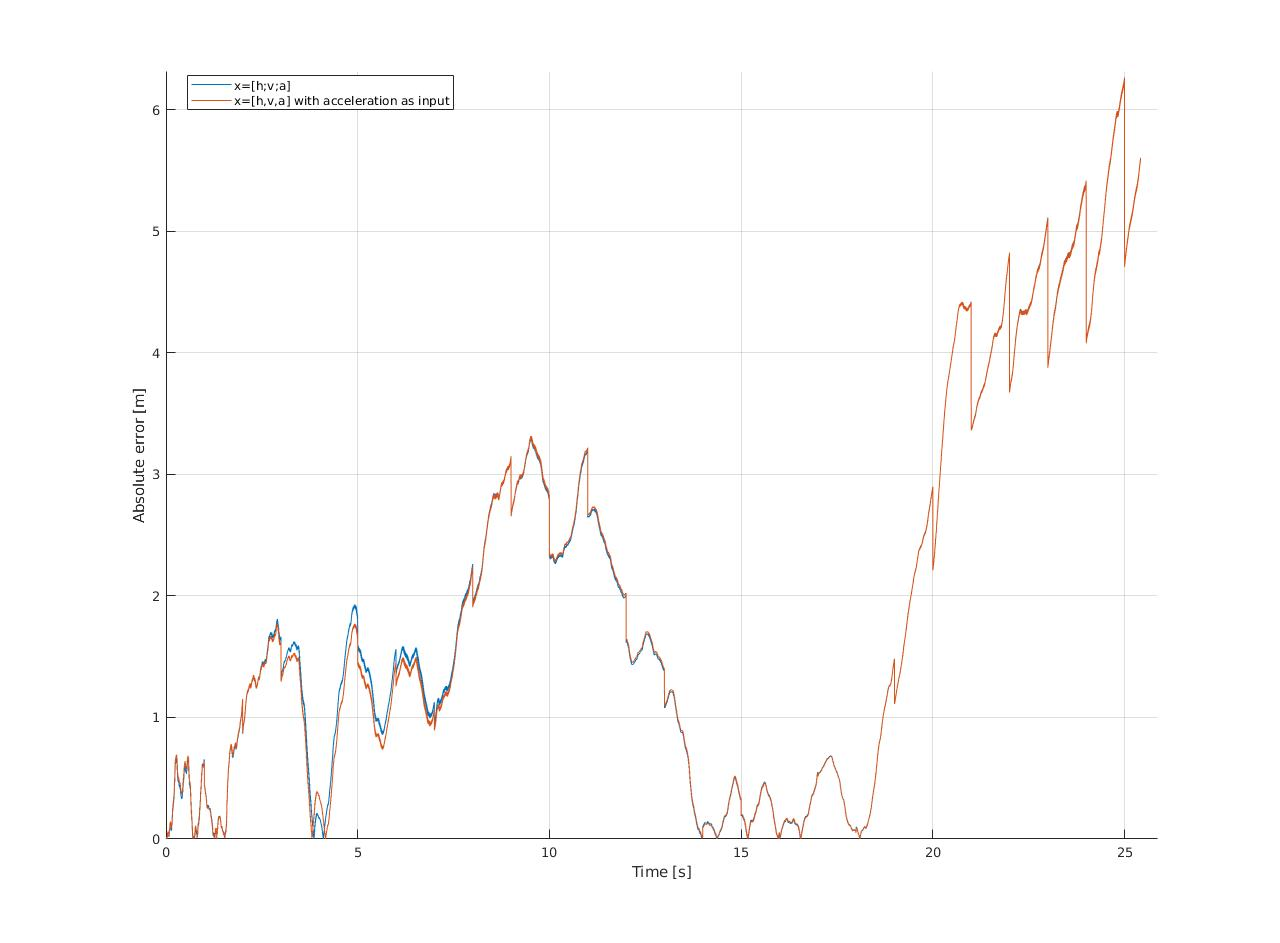
\includegraphics[width=.8\textwidth]{./Pictures/PointMassVSAccelerationInput.jpg}
 % PointMassVSAccelerationInput.jpg: 0x0 pixel, 300dpi, 0.00x0.00 cm, bb=
 \caption{Error over the flight from the point mass system model with and without the acceleration as input}
 \label{fig:PointMassVSAccelerationInput}
\end{figure}

The difference between int the errors between this system model and the normal point mass model is mostly due rounding errors of the simulation then due to really better estimation.
This can be assumed due to the fact that this system model performs some time slightly better and some time slightly worse than the point mass system-
Therefore there is no real gain in the implementation this way.
In addition with this version the additional adjustment factor which was the system noise onto the acceleration can not be used.
This means a additional parameter for tuning is lost.
So it does not really make sense to use this in the final version.


\section{Point Mass with offset and better calculated system noise}
The better calculated system noise first by accessing it in the second was stated in \ref{ch:Implementation}
This by calculating the discrete system noise matrix with the integration as well as
derive the perfect measurements and then low pass filter them to get better system noise vectors.
This had to be used on a system which uses the acceleration offset as well in the state vector to get fully possible gain out of this implemenation.
Figure \ref{fig:PointMassVSBetterNoise} shows that an over hall better estimation can be achieved with this tactic. 
\begin{figure}[h!]
 \centering
 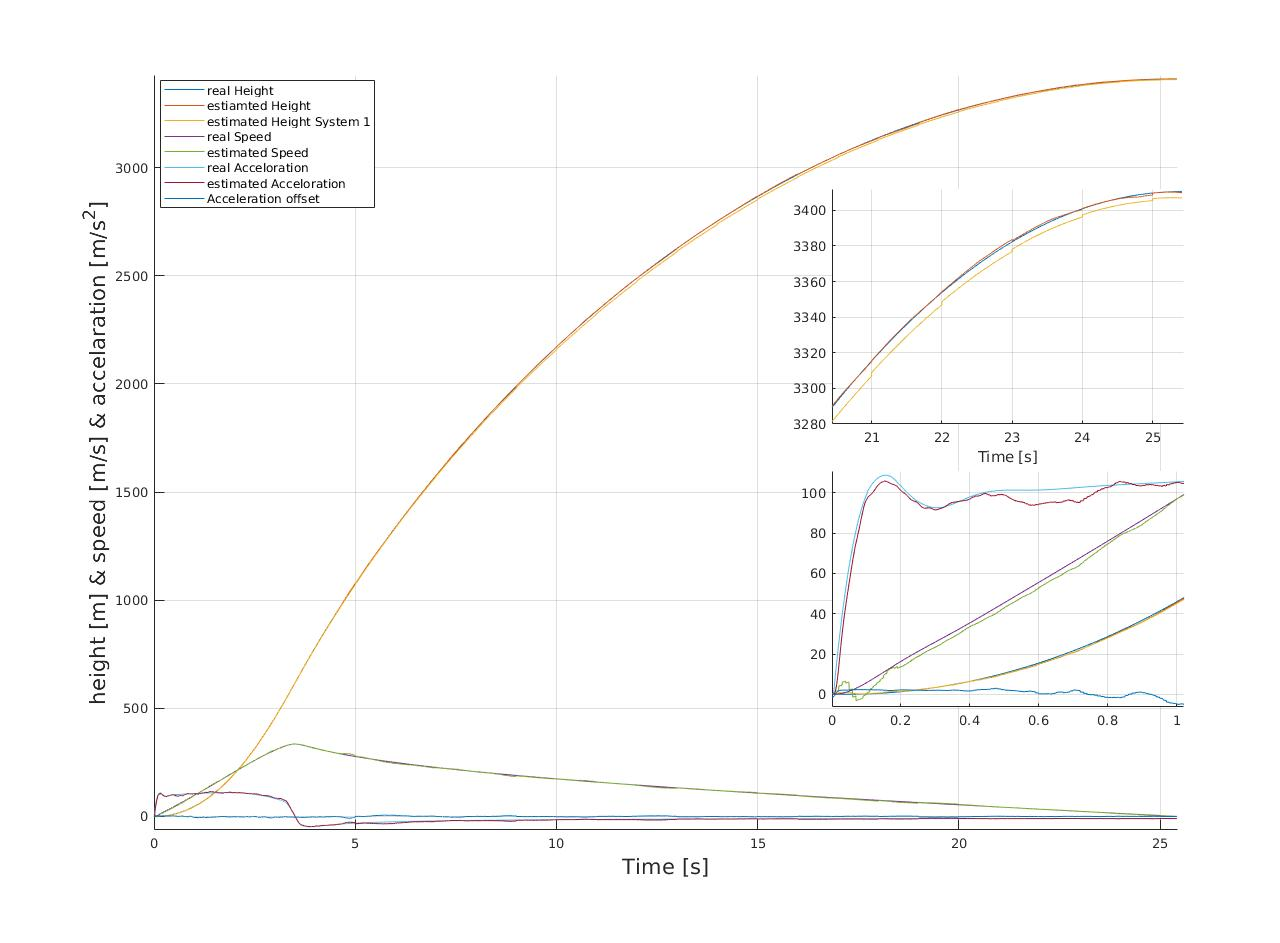
\includegraphics[width=.8\textwidth]{./Pictures/PointMassVSBetterNoise.jpg}
 % PointMassVSBetterNoise.jpg: 0x0 pixel, 300dpi, 0.00x0.00 cm, bb=
 \caption{Error over time with and without better system noise}
 \label{fig:PointMassVSBetterNoise}
\end{figure}


This mostly due the better system noise vector which are much better estimated this way.
Also the additional effort to access this system model only occurs on the preparation,
while it does have no effect on the computational effort during the flight itself.
Non the less this expansion of the state estimation should be used any time if available.

\section{With and without GPS}
It is not certain that the GPS will be working like stated before in the coming competitions.
In addition the need more time be measured and can therefore arrive to late to be included correctly.
There is the possibility back calculating to include such too late arrived measurements into the state estimation but they need a lot of calculational effort \cite{SimonDan2006Ose:}.

Because of this, the estimation without the GPS measurements are tested with a point mass system model to find its direct impacts.
Figure \ref{fig:PointMassWithWithoutGPS} shows the plot of different estimation with and without working GPS.

\begin{figure}[h!]
 \centering
 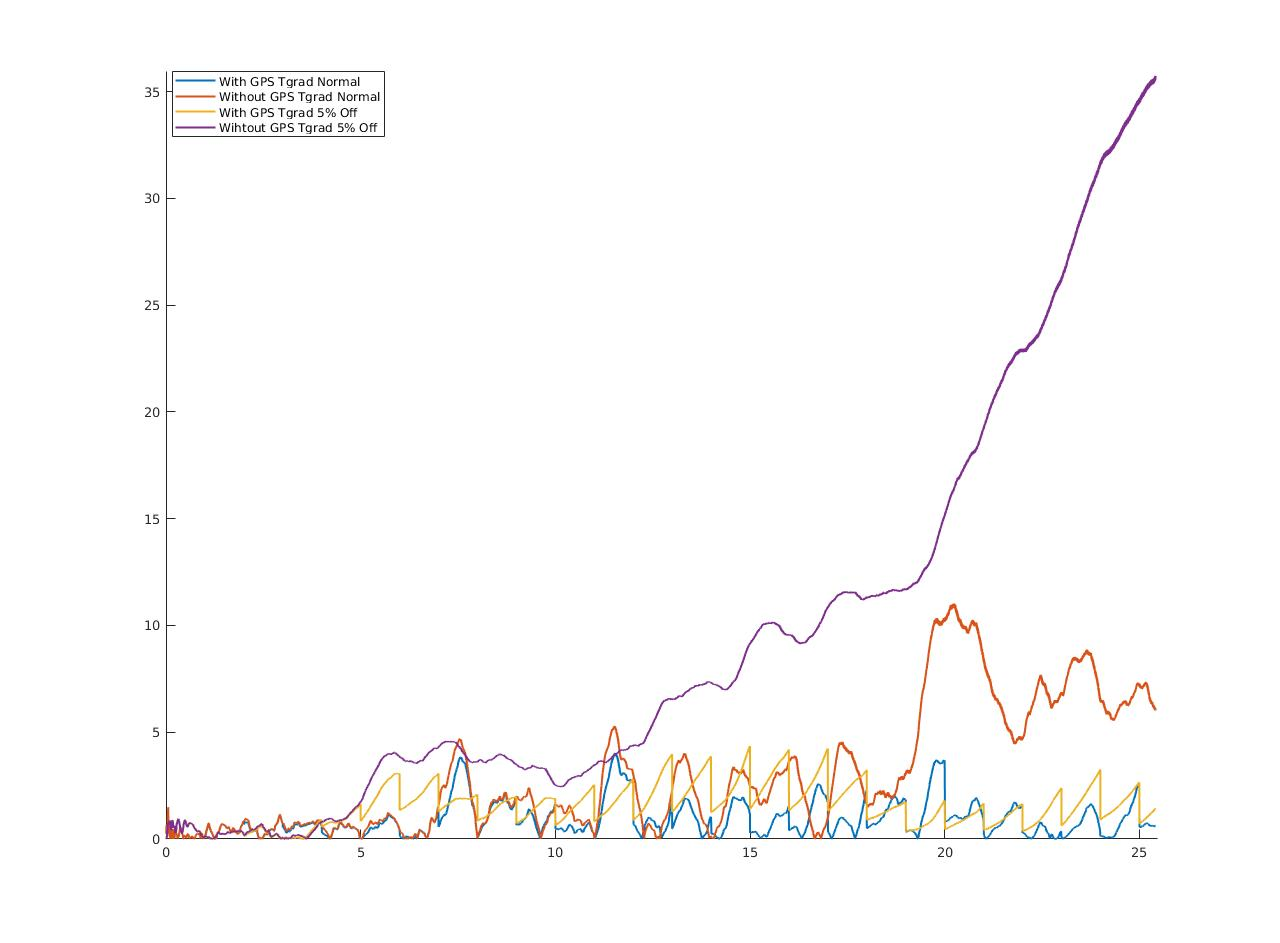
\includegraphics[width=.8\textwidth]{./Pictures/PointMassWithWithoutGPS.jpg}
 % PointMassWithWithoutGPS.jpg: 0x0 pixel, 300dpi, 0.00x0.00 cm, bb=
 \caption{Absloute error over time with and without GPS}
 \label{fig:PointMassWithWithoutGPS}
\end{figure}

It shows that especially if the temperature gradient is chosen wrong and
therefore the height out of the pressure measurements is calculated wrong the error of the estimation rises significantly.

\section{Best Performance System}
Out of the results from the test above the best fitting system can be defined.
While the pitch angle did not have a positive effect on the estimation, the effect of the pressure as a state variable is also to risky to really use it.
Also acceleration as input does not significantly improve the estimation and will therefore not be used.
Therefore the best system consist out of the additional acceleration offset as a state vector as well as better calculated system noise.

It was tested with and without GPS because it is not sure that this would function

\subsection{With GPS}

\subsection{Without GPS}

\subsection{Robustness}
The robustness is by far the most important property of the estimation.
This in the concept of being able to function if a sensor fails which will be covered below as well as being robust against false system modeling 
and especially falsely detected temperature gradients. So this will be discussed here.


\subsection{Perfomance}
Maybe in conclusion

\section{Sensor Outfall}
In addition to the test for the different system model implementation
the possibility to simulate outfalls of the different sensors at start or during the flight was implemented for the last system model.
This by setting the measurement noises of these sensors to the maximal value (represental to infinity).

\subsection{GPS Outfall}
The outfall of a GPS was also discussed above which would represent a state estimation with no GPS measurements at all.
In addition will here be discussed how the state estimation is affected if the GPS measurements are lost during the flight.

% Here comes a plot 

\subsection{Barometer Outfall}
\subsection{Accelerometer Outfall}
\subsection{Gyrometer Outfall}